\documentclass{standalone}
\usepackage{tikz}
\usetikzlibrary{patterns, positioning}
\usepackage[sfdefault]{ClearSans} %% option 'sfdefault' activates Clear Sans as the default text font
\usepackage[T1]{fontenc}

\begin{document}
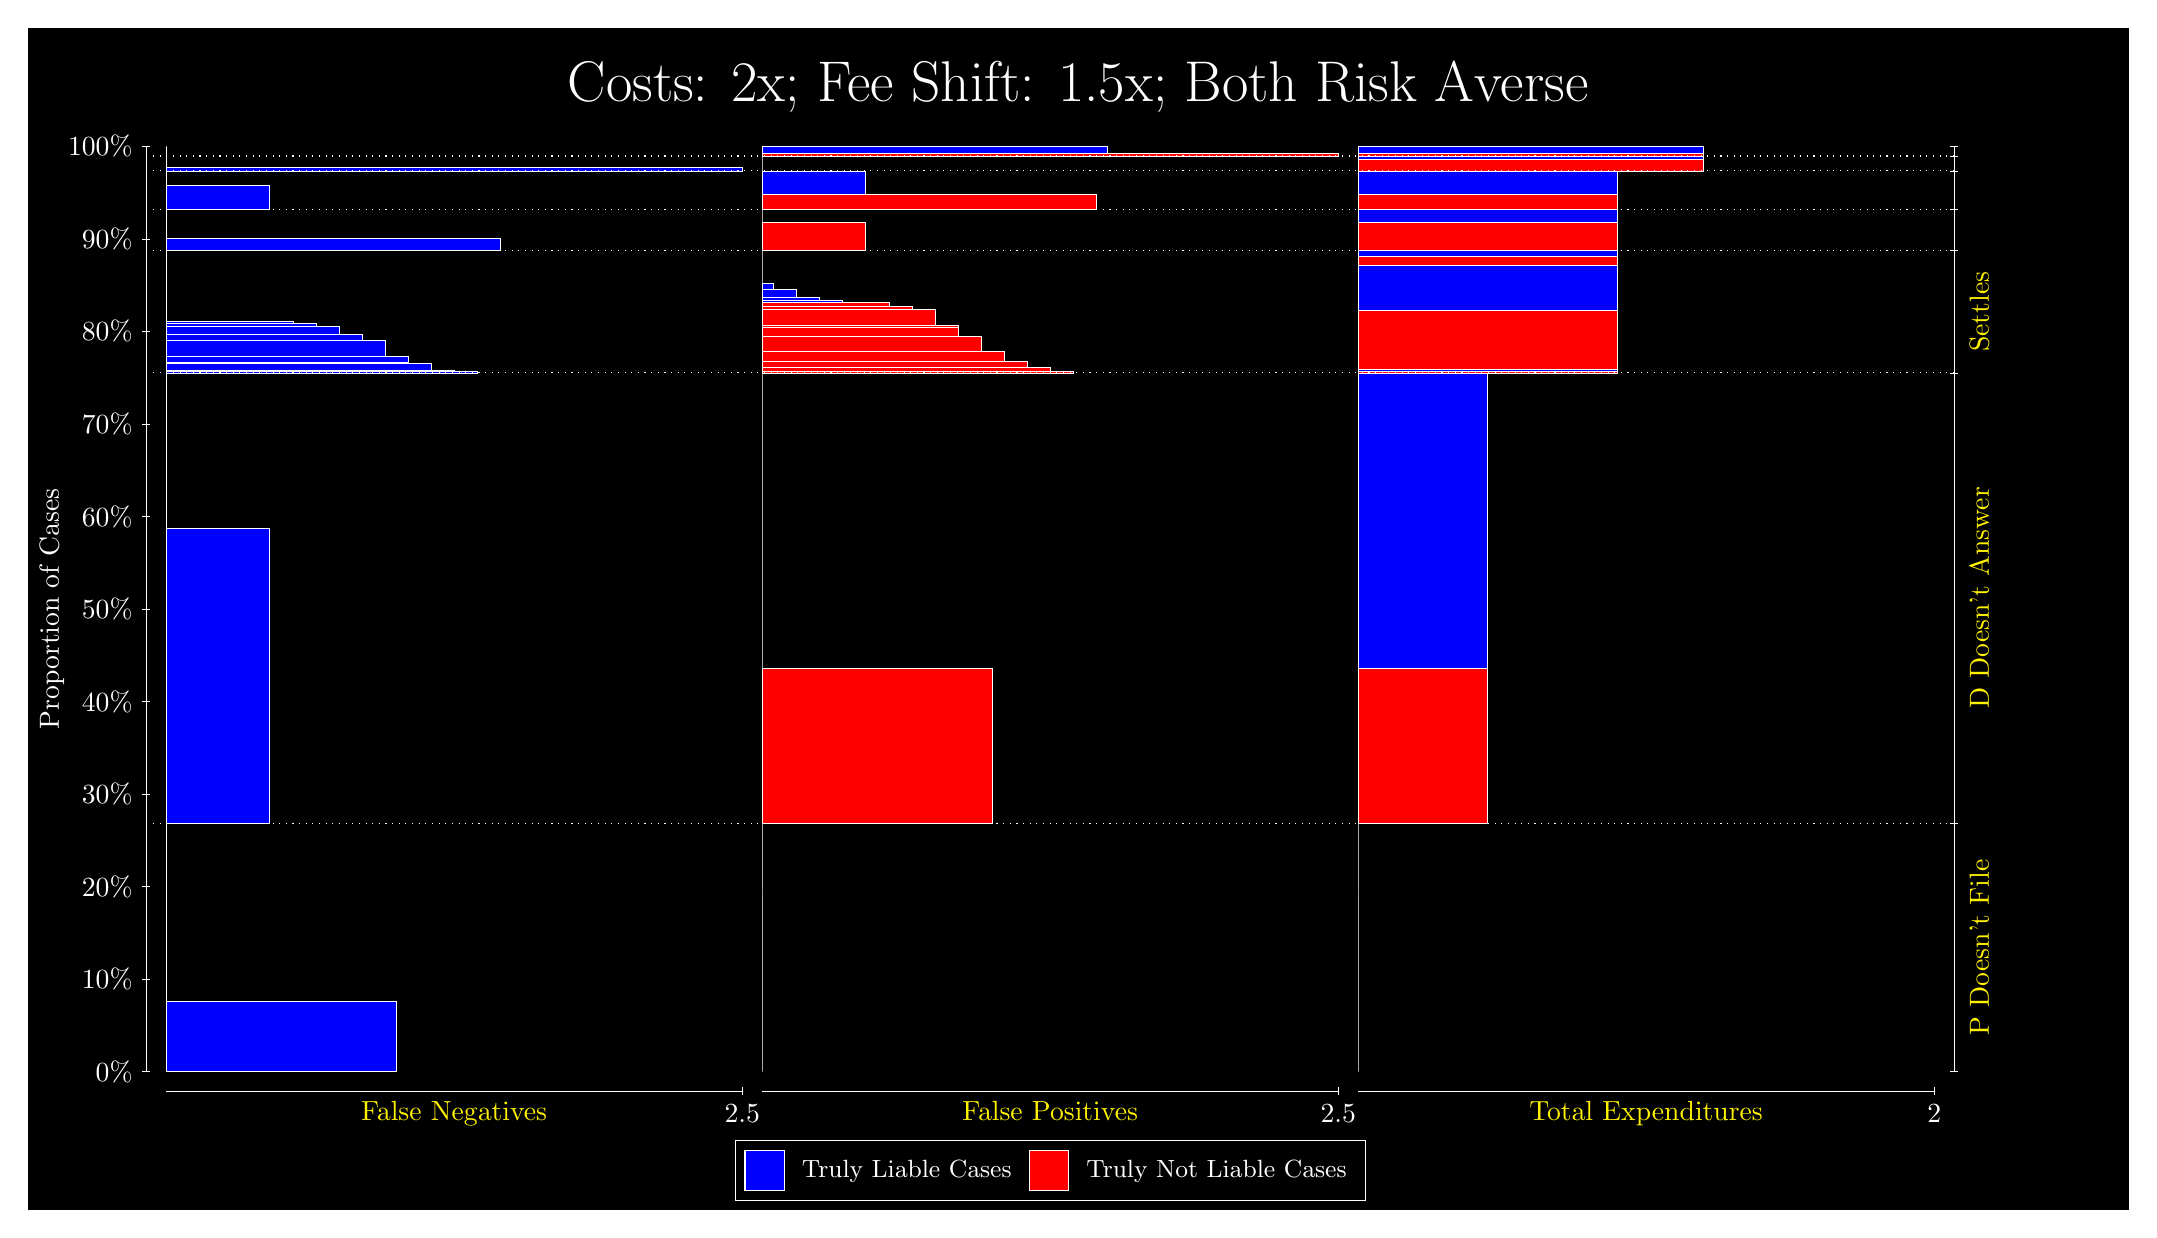
\begin{tikzpicture}
\draw[fill=black] (0,0) rectangle (26.667,15);
\draw[text=white] (0,13.5) rectangle (26.667,15) node[midway] {\huge Costs: 2x; Fee Shift: 1.5x; Both Risk Averse};
\draw[white, very thin] (1.5,1.75) -- (1.5,13.5);
\node[rotate=90, text=white, anchor=center] at (0.3, 7.625) {Proportion of Cases};
\draw[white, very thin] (1.45,1.75) -- (1.55,1.75);
\node[text=white, anchor=east] at (1.45, 1.75) {0\%};
\draw[white, very thin] (1.45,2.925) -- (1.55,2.925);
\node[text=white, anchor=east] at (1.45, 2.925) {10\%};
\draw[white, very thin] (1.45,4.1) -- (1.55,4.1);
\node[text=white, anchor=east] at (1.45, 4.1) {20\%};
\draw[white, very thin] (1.45,5.275) -- (1.55,5.275);
\node[text=white, anchor=east] at (1.45, 5.275) {30\%};
\draw[white, very thin] (1.45,6.45) -- (1.55,6.45);
\node[text=white, anchor=east] at (1.45, 6.45) {40\%};
\draw[white, very thin] (1.45,7.625) -- (1.55,7.625);
\node[text=white, anchor=east] at (1.45, 7.625) {50\%};
\draw[white, very thin] (1.45,8.8) -- (1.55,8.8);
\node[text=white, anchor=east] at (1.45, 8.8) {60\%};
\draw[white, very thin] (1.45,9.975) -- (1.55,9.975);
\node[text=white, anchor=east] at (1.45, 9.975) {70\%};
\draw[white, very thin] (1.45,11.15) -- (1.55,11.15);
\node[text=white, anchor=east] at (1.45, 11.15) {80\%};
\draw[white, very thin] (1.45,12.325) -- (1.55,12.325);
\node[text=white, anchor=east] at (1.45, 12.325) {90\%};
\draw[white, very thin] (1.45,13.5) -- (1.55,13.5);
\node[text=white, anchor=east] at (1.45, 13.5) {100\%};

\draw[white, very thin] (24.457,1.75) -- (24.457,13.5);
\draw[white, very thin] (24.407,1.75) -- (24.507,1.75);
\node[anchor=west] at (24.407, 1.75) {};
\draw[white, very thin] (24.407,4.9033) -- (24.507,4.9033);
\node[anchor=west] at (24.407, 4.9033) {};
\draw[white, very thin] (24.407,10.624) -- (24.507,10.624);
\node[anchor=west] at (24.407, 10.624) {};
\draw[white, very thin] (24.407,12.175) -- (24.507,12.175);
\node[anchor=west] at (24.407, 12.175) {};
\draw[white, very thin] (24.407,12.699) -- (24.507,12.699);
\node[anchor=west] at (24.407, 12.699) {};
\draw[white, very thin] (24.407,13.188) -- (24.507,13.188);
\node[anchor=west] at (24.407, 13.188) {};
\draw[white, very thin] (24.407,13.377) -- (24.507,13.377);
\node[anchor=west] at (24.407, 13.377) {};
\draw[white, very thin] (24.407,13.5) -- (24.507,13.5);
\node[anchor=west] at (24.407, 13.5) {};

\draw[white, very thin, fill=blue] (1.75,1.75) rectangle (4.6775,2.6418);
\draw[white, very thin, fill=red] (1.75,2.6418) rectangle (1.75,4.9033);
\draw[white, very thin, fill=blue] (1.75,4.9033) rectangle (3.0674,8.6501);
\draw[white, very thin, fill=red] (1.75,8.6501) rectangle (1.75,10.624);
\draw[white, very thin, fill=blue] (1.75,10.624) rectangle (5.7022,10.643);
\draw[white, very thin, fill=blue] (1.75,10.643) rectangle (5.4094,10.662);
\draw[white, very thin, fill=blue] (1.75,10.662) rectangle (5.1167,10.746);
\draw[white, very thin, fill=blue] (1.75,10.746) rectangle (4.8239,10.759);
\draw[white, very thin, fill=blue] (1.75,10.759) rectangle (4.8239,10.833);
\draw[white, very thin, fill=blue] (1.75,10.833) rectangle (4.5312,11.038);
\draw[white, very thin, fill=blue] (1.75,11.038) rectangle (4.2384,11.112);
\draw[white, very thin, fill=blue] (1.75,11.112) rectangle (3.9457,11.21);
\draw[white, very thin, fill=blue] (1.75,11.21) rectangle (3.6529,11.259);
\draw[white, very thin, fill=blue] (1.75,11.259) rectangle (3.3602,11.277);
\draw[white, very thin, fill=red] (1.75,11.277) rectangle (1.75,12.175);
\draw[white, very thin, fill=blue] (1.75,12.175) rectangle (5.9949,12.335);
\draw[white, very thin, fill=red] (1.75,12.335) rectangle (1.75,12.699);
\draw[white, very thin, fill=blue] (1.75,12.699) rectangle (3.0674,12.999);
\draw[white, very thin, fill=red] (1.75,12.999) rectangle (1.75,13.188);
\draw[white, very thin, fill=blue] (1.75,13.188) rectangle (9.0689,13.228);
\draw[white, very thin, fill=red] (1.75,13.228) rectangle (1.75,13.377);
\draw[white, very thin, fill=red] (1.75,13.377) rectangle (1.75,13.417);
\draw[white, very thin, fill=blue] (1.75,13.417) rectangle (1.75,13.5);
\draw[white, very thin, fill=red] (9.3189,1.75) rectangle (9.3189,4.0115);
\draw[white, very thin, fill=blue] (9.3189,4.0115) rectangle (9.3189,4.9033);
\draw[white, very thin, fill=red] (9.3189,4.9033) rectangle (12.246,6.8771);
\draw[white, very thin, fill=blue] (9.3189,6.8771) rectangle (9.3189,10.624);
\draw[white, very thin, fill=red] (9.3189,10.624) rectangle (13.271,10.648);
\draw[white, very thin, fill=red] (9.3189,10.648) rectangle (12.978,10.69);
\draw[white, very thin, fill=red] (9.3189,10.69) rectangle (12.686,10.775);
\draw[white, very thin, fill=red] (9.3189,10.775) rectangle (12.393,10.893);
\draw[white, very thin, fill=red] (9.3189,10.893) rectangle (12.1,11.082);
\draw[white, very thin, fill=red] (9.3189,11.082) rectangle (11.807,11.208);
\draw[white, very thin, fill=red] (9.3189,11.208) rectangle (11.807,11.231);
\draw[white, very thin, fill=red] (9.3189,11.231) rectangle (11.515,11.426);
\draw[white, very thin, fill=red] (9.3189,11.426) rectangle (11.222,11.473);
\draw[white, very thin, fill=red] (9.3189,11.473) rectangle (10.929,11.522);
\draw[white, very thin, fill=blue] (9.3189,11.522) rectangle (10.344,11.54);
\draw[white, very thin, fill=blue] (9.3189,11.54) rectangle (10.051,11.589);
\draw[white, very thin, fill=blue] (9.3189,11.589) rectangle (9.758,11.687);
\draw[white, very thin, fill=blue] (9.3189,11.687) rectangle (9.4652,11.761);
\draw[white, very thin, fill=blue] (9.3189,11.761) rectangle (9.3189,12.175);
\draw[white, very thin, fill=red] (9.3189,12.175) rectangle (10.636,12.539);
\draw[white, very thin, fill=blue] (9.3189,12.539) rectangle (9.3189,12.699);
\draw[white, very thin, fill=red] (9.3189,12.699) rectangle (13.564,12.888);
\draw[white, very thin, fill=blue] (9.3189,12.888) rectangle (10.636,13.188);
\draw[white, very thin, fill=red] (9.3189,13.188) rectangle (9.3189,13.337);
\draw[white, very thin, fill=blue] (9.3189,13.337) rectangle (9.3189,13.377);
\draw[white, very thin, fill=red] (9.3189,13.377) rectangle (16.638,13.417);
\draw[white, very thin, fill=blue] (9.3189,13.417) rectangle (13.71,13.5);
\draw[white, very thin, fill=red] (16.888,1.75) rectangle (16.888,4.0115);
\draw[white, very thin, fill=blue] (16.888,4.0115) rectangle (16.888,4.9033);
\draw[white, very thin, fill=red] (16.888,4.9033) rectangle (18.534,6.8771);
\draw[white, very thin, fill=blue] (16.888,6.8771) rectangle (18.534,10.624);
\draw[white, very thin, fill=red] (16.888,10.624) rectangle (20.181,10.648);
\draw[white, very thin, fill=blue] (16.888,10.648) rectangle (20.181,10.665);
\draw[white, very thin, fill=red] (16.888,10.665) rectangle (20.181,11.422);
\draw[white, very thin, fill=blue] (16.888,11.422) rectangle (20.181,11.983);
\draw[white, very thin, fill=red] (16.888,11.983) rectangle (20.181,12.101);
\draw[white, very thin, fill=blue] (16.888,12.101) rectangle (20.181,12.175);
\draw[white, very thin, fill=red] (16.888,12.175) rectangle (20.181,12.539);
\draw[white, very thin, fill=blue] (16.888,12.539) rectangle (20.181,12.699);
\draw[white, very thin, fill=red] (16.888,12.699) rectangle (20.181,12.888);
\draw[white, very thin, fill=blue] (16.888,12.888) rectangle (20.181,13.188);
\draw[white, very thin, fill=red] (16.888,13.188) rectangle (21.279,13.337);
\draw[white, very thin, fill=blue] (16.888,13.337) rectangle (21.279,13.377);
\draw[white, very thin, fill=red] (16.888,13.377) rectangle (21.279,13.417);
\draw[white, very thin, fill=blue] (16.888,13.417) rectangle (21.279,13.5);
\draw[white, dotted] (1.5,4.9033) -- (24.457,4.9033);
\draw[white, dotted] (1.5,10.624) -- (24.457,10.624);
\draw[white, dotted] (1.5,12.175) -- (24.457,12.175);
\draw[white, dotted] (1.5,12.699) -- (24.457,12.699);
\draw[white, dotted] (1.5,13.188) -- (24.457,13.188);
\draw[white, dotted] (1.5,13.377) -- (24.457,13.377);
\draw[white, very thin] (1.75,1.5) -- (9.0689,1.5);
\node[text=yellow, anchor=north] at (5.4094, 1.5) {False Negatives};
\draw[white, very thin] (9.0689,1.45) -- (9.0689,1.55);
\node[text=white, anchor=north] at (9.0689, 1.45) {2.5};

\draw[white, very thin] (9.3189,1.5) -- (16.638,1.5);
\node[text=yellow, anchor=north] at (12.978, 1.5) {False Positives};
\draw[white, very thin] (16.638,1.45) -- (16.638,1.55);
\node[text=white, anchor=north] at (16.638, 1.45) {2.5};

\draw[white, very thin] (16.888,1.5) -- (24.207,1.5);
\node[text=yellow, anchor=north] at (20.547, 1.5) {Total Expenditures};
\draw[white, very thin] (24.207,1.45) -- (24.207,1.55);
\node[text=white, anchor=north] at (24.207, 1.45) {2};

\node[text=yellow, centered, rotate=90] at (24.777, 3.3267) {P Doesn't File};
\node[text=yellow, centered, rotate=90] at (24.777, 7.7636) {D Doesn't Answer};
\node[text=yellow, centered, rotate=90] at (24.777, 11.4) {Settles};





\draw (12.978300999999998,1.5) node[draw=none] (baseCoordinate) {};
\begin{scope}[align=center]
        \matrix[scale=0.5, draw=white, below=0.5cm of baseCoordinate, nodes={draw}, column sep=0.1cm]{
            \node[rectangle, draw, minimum width=0.5cm, minimum height=0.5cm, fill=blue] {}; &
            \node[draw=none, font=\small, text=white] (B) {Truly Liable Cases}; &
            \node[rectangle, draw, minimum width=0.5cm, minimum height=0.5cm, fill=red] {}; &
            \node[draw=none, font=\small, text=white] (B) {Truly Not Liable Cases}; \\
            };
\end{scope}

\end{tikzpicture}
\end{document}